\chapter{Experiments}\label{chp:experiments}

In this chapter we'll benchmark a WebRTC-based video conferencing solution for our test cases, to get a sense of how a peer-to-peer architecture performs.


\section{Test Setup}

To benchmark appear.in, our WebRTC-based video conferencing solution of choice, we have utilized a small cluster of desktop computers with web cameras, running the most recent versions of Mozilla Firefox\footnote{Version 36.0.4, latest version as of 2015.06.05 when the tests were run} and Google Chrome\footnote{Version 41.0.2272.101, latest version as of 2015.06.11 when the tests were run}. These two browsers were chosen since they collectively represent 85\% of the browser market (according to both appear.in data as seen in \autoref{chp:appear.in-usage} and the W3C \cite{browser-stats}), and are powered by two different underlying engines. The goal of the benchmark is to get a sense of how the browsers -- and by extension, appear.in -- performs with regard to latency and bandwidth usage in our different test scenarios, and from that data observe how resources are shared among the nodes in a conversation.

Since the test covers two different browsers which do not share a common API (more on this later), measurements were done in two different ways. For Firefox, which do not expose timing data of WebRTC-streams, a browser-external way of measuring end-to-end latencies was necessary. For this we synchronized all the clocks in the cluster to the same \gls{NTP} server, and set another independent node -- also synced to the same time server -- to run a timer. Each of the nodes in the test filmed this timer, and with the same timer running locally in a terminal, the end-to-end latency could be extracted by taking regular screenshots, and finding the difference between the local timer and the timer as sent by the other nodes. See \autoref{fig:example-screenshot} for an example of how the screenshots looked.

\begin{figure}
    \centering
    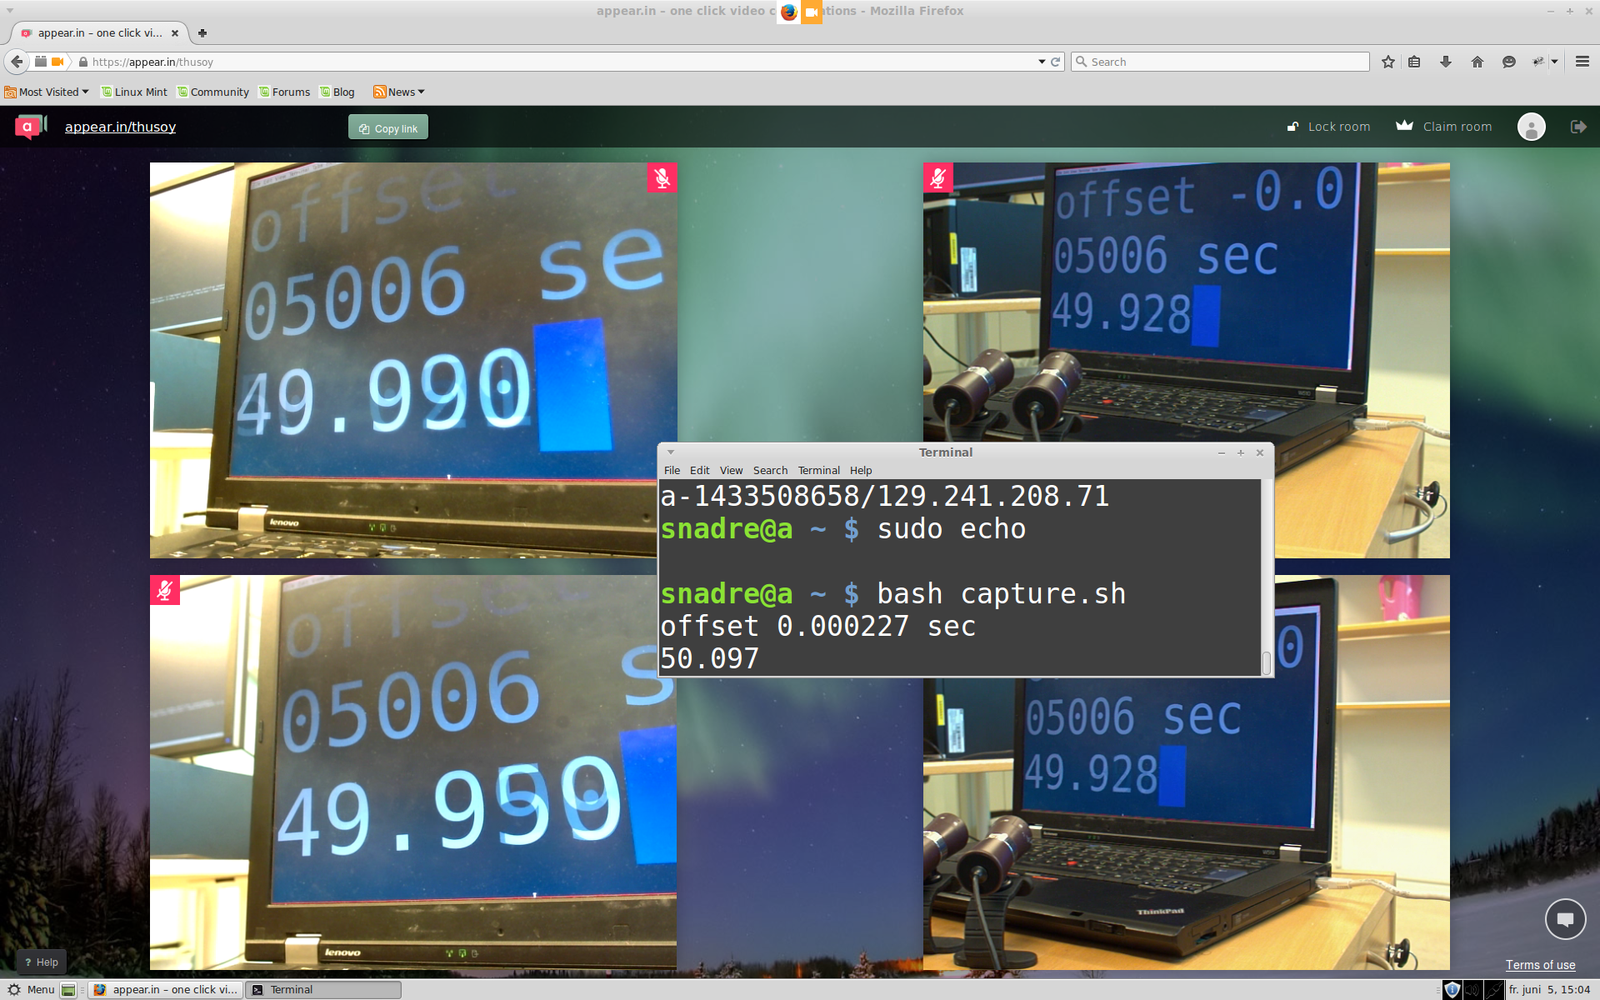
\includegraphics[width=.7\textwidth]{example-screenshot}
    \caption{An example screenshot from a test run on node A. The nodes are, from top left and clockwise, A, C, B and D. We can see from the difference between the local timestamp and A's own video stream that there's about 75ms of processing time in the browser before the image is sent (if we round A up to the almost visible 50.021 timestamp), and that the latencies from the other nodes are 31ms, 93ms and 93ms for B, C, and D, respectively.}
    \label{fig:example-screenshot}
\end{figure}

Bandwidth usage was measured by running \texttt{tcpdump} throughout the test run, and later extracting sent and received data with \texttt{tshark}.

For the Chrome tests, this was a bit simpler and less manual, as Chrome do provider timing data through the \texttt{getStats} API. Firefox also supports \texttt{getStats}, but does not return as much data as Chrome does, even though the data is assumed to be available internally in the browser.


\subsection{Sampling}

At the start of the test, the nodes join the conversation in alphabetical order (the node names are letters A-G), as soon as the previous node has established connection to all the other parties already in the conversation. Preferably the join order would be random and the results averaged over several test runs, but due to time constraints this was not possible.

When all nodes have established bi-directional connections, the conversation was left running for a minute, before sampling started. This was done to allow some time to reach a stable state.

For Firefox, where the interpretation of the results is a very tedious and laboursome process, samples were taken every $\approx$12s\footnote{A bit variable, as it's 10s + the delay for taking and storing the screenshot}. The last six samples for each node was interpreted and stored, yielding a total sample time of $\approx$80s. On Chrome, were there's no interpretation step, samples were submitted every second, and the sample time was two minutes, yielding 120 samples for each node.

For all test cases the test was first run without any traffic shaping applied, so that the actual test results could be seen in comparison to results without any network limitations.


\subsection{getStats}

The relevant values offered by the \texttt{getStats}-API on Chrome\footnote{Documentation is very poor for the \texttt{getStats}-API, as the specification is not completed yet, so the most reliable reference is the source: \url{https://chromium.googlesource.com/external/webrtc/+/master/talk/app/webrtc/statstypes.cc}} and Firefox is presented in \autoref{tab:incoming-video} and \autoref{tab:outgoing-video}. The values reported here were dumped from what's returned by the browser.

\begin{center}
    \captionof{table}{Incoming video data}
    \label{tab:incoming-video}
    \begin{tabular}{| l | l |}
        \hline
        \textbf{Chrome} & \textbf{Firefox} \\ \hline
        \multicolumn{2}{| c |}{bytesReceived:\texttt{str/int}} \\
        \multicolumn{2}{| c |}{packetsLost:\texttt{str/int}} \\
        \multicolumn{2}{| c |}{packetsReceived:\texttt{str/int}} \\ \hline
        googCurrentDelayMs:\texttt{str} & jitter:\texttt{float} \\
        googDecodeMs:\texttt{str} & mozRtt:\texttt{int} \\
        googJitterBufferMs:\texttt{str} & \\
        googMaxDecodeMs:\texttt{str} & \\
        googMinPlayoutDelayMs:\texttt{str} & \\
        googRenderDelayMs:\texttt{str} & \\
        googTargetDelayMs:\texttt{str} & \\ \hline
    \end{tabular}
\end{center}

\begin{center}
    \captionof{table}{Outgoing video data}
    \label{tab:outgoing-video}
    \begin{tabular}{| l | l |}
        \hline
        \textbf{Chrome} & \textbf{Firefox} \\ \hline
        \multicolumn{2}{| c |}{bytesSent:\texttt{str/int}} \\
        \multicolumn{2}{| c |}{packetsSent:\texttt{str/int}} \\ \hline
        googAvgEncodeMs:\texttt{str} & bitrateMean:\texttt{float} \\
        googCaptureJitterMs:\texttt{str} & bitrateStdDev:\texttt{float} \\
        googCaptureQueueDelayMsPerS:\texttt{str} & droppedFrames:\texttt{int} \\
        googCodecName:\texttt{str} & framerateMean:\texttt{float} \\
        googBandwidthLimitedResolution:\texttt{str} & framerateStdDev:\texttt{float} \\
        googCpuLimitedResolution:\texttt{str} & \\
        googViewLimitedResolution:\texttt{str} & \\
        googRtt:\texttt{str} & \\
        packetsLost:\texttt{str} & \\ \hline
    \end{tabular}
\end{center}

It's a bit sad to see that all of the values are casted to strings in Chrome. This is not the case on Firefox, where appropriate types are used. As we also see, all of the timing-related values we're interested are vendor-prefixed on Chrome, which hints to their unspecified nature. Note that both browsers report more data than what is shown here, this is only the data I consider to be relevant for our bandwidth and latency measurements (and link quality, thus the ones related to packet loss). Chrome is also very helpful in providing why resolution is limited (received resolution is present in the full data set), which could be incorporated into more advanced models.


\subsection{Constraining Nodes}

To configure the cluster according to the different test cases, we utilized the Linux traffic control utility \texttt{tc}, which is capable of rate-limiting incoming and outgoing traffic, as well as delaying traffic destined for certain hosts. A small script was developed to act as a glue layer between a representation of a network and \texttt{tc}, making configuration repeatable and easily parametrized. The script is included in \autoref{chp:apply-case}.

Thus, applying a given test case is completely independent of the actual network utilized in the test cluster, keeping all intelligence on the nodes themselves. This removed the need for expensive routers or having to customize the application code, thus making the method application agnostic and applicable to any peer-to-peer solution, not just appear.in.


\subsection{Automated Testing?}\label{subsec:automated-testing}

Ideally, testing would be automated and not require a running graphical environment, to allow tests to be run often and in response to events such as commits. This could be possible using by running a browser in a fake framebuffer like \texttt{Xvfb}\footnote{\url{http://www.x.org/releases/X11R7.6/doc/man/man1/Xvfb.1.xhtml}} and faking out a media stream\footnote{Chrome: \texttt{-{}-use-fake-device-for-media-stream}, Firefox: \texttt{getUserMedia(\{fake: true, <...>\})}. More info about this approach can be found at \url{http://images.tmcnet.com/expo/webrtc-conference/presentations/san-jose-14/D3-2_Testing_v2_2.pdf}}. Both browsers should be able to be tested in such a setting, but data would be limited to what can be extracted through the \texttt{getStats}-API as described above. Still, it's better than nothing. It is thus possible to automate this, but was considered out of scope for this thesis.


\subsection{Caveats}

The Firefox method is accurate in the sense that latencies observed are the actual end-to-end latencies that users would observe, but the precision of the timing values observed is not on the millisecond level we'd prefer. This is due to a number of factors, most notably the refresh rate of the screen running the timer and the framerate of the video, limiting the precision to $1s/60\approx17ms$ and $1s/30\approx33ms$ respectively. However, we can surpass this precision by averaging several samples taken during the test run, which is why we take several screenshots for each test case, once every 10s for at least a minute. The standard deviation of the measurements is reported in the graphs included later in this chapter, which should give some indication towards how accurate the average is.

Taking several samples to improve accuracy leads us to another weakness, which is the manual interpretation of the screenshots. Due to the frequency-related issues discussed above, many of the images include timestamps that are blurred, as the camera captured two underlying screen updates in the same frame, as shown in \autoref{fig:blurred-capture}.

\begin{figure}
    \centering
    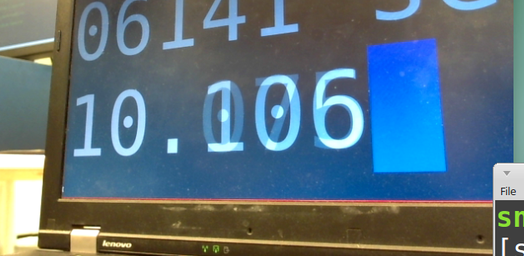
\includegraphics[width=.7\textwidth]{blurred-capture}
    \caption{A screenshot where a node has sent two overlaying timestamps. In this case interpreted as 10.106, which is reasonable as it's close to the expected 33ms increase from the previous 10.075.}
    \label{fig:blurred-capture}
\end{figure}

In general for these cases, the recorded timestamp was consistently interpreted to be the latest of what could be distinguished in the screenshot.

Even assuming that the timestamps are comprehensible and fairly accurate, there's still a possibility of human error when lots of numbers has to be recorded in this way. To minimize the risk of any mistyped numbers making it into the dataset, any number outside 1.5 standard deviations of the mean (a range which should include 87\% of the numbers observed) was verified once more. There's still a chance of smaller errors making it into the dataset, but we assume that these are small enough and distributed evenly among the nodes to not significantly influence any conclusions drawn.

As not enough cameras of any single model was available for the experiments, two different models\todo{Insert picture of the cameras here, or footnote} had to be used. These had slightly different performance characteristics; the cameras were put side by side with a timer and showed a mean difference of 39.6ms, but with a relatively large standard deviation of 19.5ms. As the same restrictions on screen refresh rates as discussed above, pretty much all the samples were at a 30ms or 60ms interval of each other.\footnote{Out of 20 samples, 1 was 0ms, 13 were 30ms, 5 were 60ms, and 1 was 90ms. Which really means in the range of that frame, that is in the range of 0--29ms difference, 30--60ms difference, and so on.} As the difference was assumed to be normally distributed, the mean was simply added to all measurements from the slower camera model to compensate.

For measuring bandwidth utilization between nodes, our method of using \texttt{tcpdump} is not entirely satisfactory, as there's no way to report actual \emph{consumed} bandwidth by the application. This is because the traffic control features of the Linux kernel lies above \texttt{libpcap}, the library that performs packet capture for \texttt{tcpdump} in the network stack. Effectively this means that any incoming bandwidth reported by \texttt{libpcap} will be before the rate limiting performed by \texttt{tc}. Thus, \texttt{tcpdump} cannot report the actual bandwidth consumed by application, only what was received by the network interface. Nonetheless, the bandwidth \emph{sent} by each node is what was actually sent by the application, but there's no guarantee that the receiver was capable of consuming it all. This is good enough for us though, as we can aggregate the data sent by all nodes to determine how saturated a given node's network link is.

While the method itself is application-agnostic, configuring nodes the way we do is not suitable for testing other architectures, such as the ones used by Hangouts and Skype. This is unfortunate, as a performance comparison between the different architectures would have been very interesting, but without running a local instance of the architecture under test, there's no way to achieve the inter-node latencies we desire. This follows from observing that if node A sends her video stream to a Google server, there's no way for her to signal to Google that when the stream is broadcast to nodes B and C, B's stream should be delayed by $x$ ms, and the stream to C should be delayed $y$ ms. It's also not possible for B and C to apply this latency on the receiving side, as they'd have to split the incoming stream for Google into separate streams for each of the transmitting nodes, which would require both getting access to the DTLS keys used by the web browser to encrypt the traffic, and being capable of splitting the stream and rejoining it again without interfering with the browser.

For the most accurate comparison of bitrate, it would have been preferable to use the same method for sampling this on both browsers. However, as Firefox was incapable of delivering timing data, the \texttt{getStats} API was discarded entirely, even though it could have been used to sample bitrates as observed by the application. This is unfortunate, but the tools left behind by these experiments allow others who want to repeat the tests to not do this mistake.


\section{Results}

\subsection{How To Read the Graphs}

As there will be a lot of graphs in this chapter, a good understanding of how to read them is essential. \autoref{fig:graph-tutorial} gives you a quick primer.

\begin{figure}
    \centering
    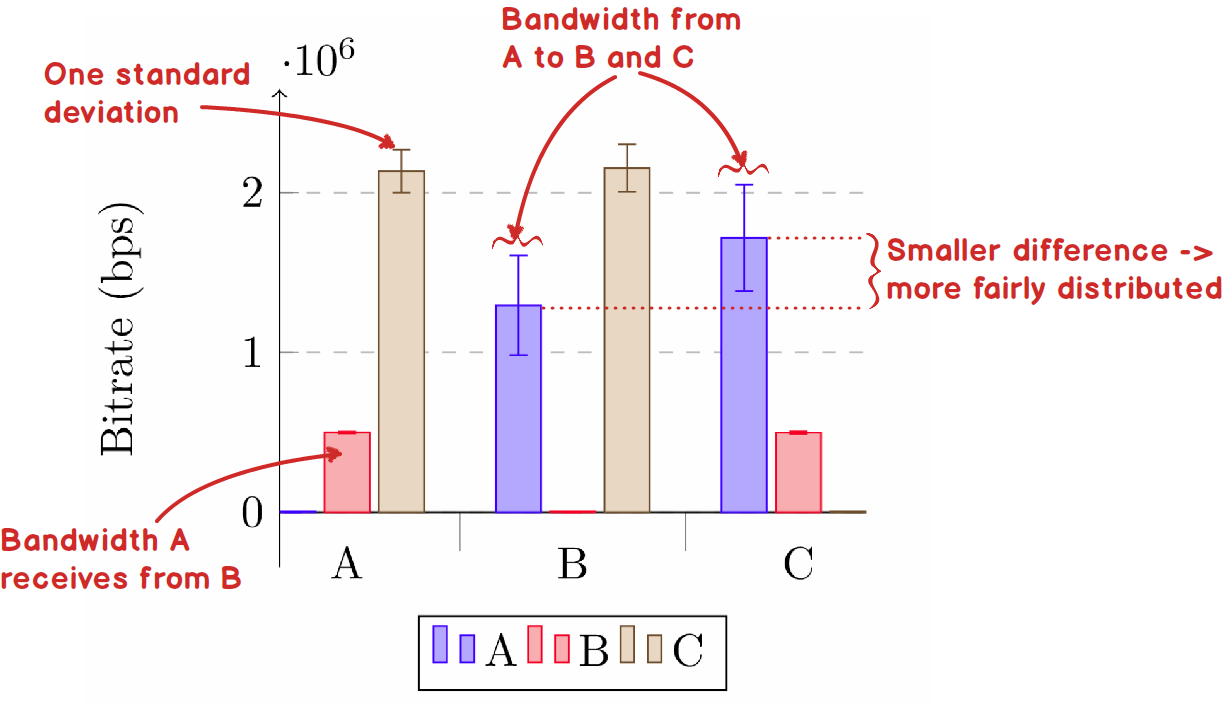
\includegraphics[width=\textwidth]{graph-tutorial}
    \caption{How to read bandwidth graphs. Latency graphs are the same, just different units.}
    \label{fig:graph-tutorial}
\end{figure}

For each node on the x-axis, if it's a latency chart the node's happier the more of the latencies are low. If it's a bitrate chart, the node's happier the more of the bars are high.

Before we embark on the test cases, we put our two sampling methods up against each other, to see whether the results are comparable. For each of the conversation sizes, 3, 4, and 7, the results were equal across the board for both browsers. Both had a consistent stable bandwidth at slightly less than 2.1Mbps, and latencies below 200ms (Chrome slightly less). The results are included in \autoref{no-shaping-comp}.

\todo[inline]{[minor] If time, define custom color set for graphing, based possibly either on solarized or http://clrs.cc/}

\subsubsection{Test Case ``traveller''}

A quick recap of the bandwidth limits put on the nodes in the ``traveller'' test case: A (10/5), B (2/1), C (10/8).

\autoref{fig:traveller-bitrate} shows the bitrates flowing between the nodes in the ``traveller'' test case. Remember what was mentioned earlier; the values reported here are only what was received at the node's interface, not what the application was consuming. This is important, as it seems from the bandwidths alone that everyone is doing fairly well in the Firefox case; but look closer. Node B only has a 2Mbps downlink, but is sent more than 3Mbps of data. Thus its link is completely saturated, which is again reflected in the latencies in \autoref{fig:traveller-latency}. We can also see that node B is saturating its own uplink as well, which also has a grave impact on the latencies.

Chrome balances this out much better, where A and C communicate unhindered by the constraints of node B (like the Firefox case), but also respect B's constraints and only send what it's capable of receiving. Thus, B's downlink has $\approx$50\% utilization, and likewise $\approx$66\% for the uplink.

\begin{figure}
    \centering
    \begin{subfigure}[t]{.48\textwidth}
        \centering
        \begin{tikzpicture}
        \begin{axis}[
            ybar,
            ylabel=Bitrate (bps),
            xtick=data,
            width=\textwidth,
            symbolic x coords={A,B,C},
            enlargelimits=0.15,
            major grid style=dashed,
            ymajorgrids,
            ]
            \input{data/appear.in-traveller/bitrate.tex}
        \end{axis}
        \end{tikzpicture}
        \subcaption{Firefox}
    \end{subfigure}
    \hfill
    \begin{subfigure}[t]{.48\textwidth}
        \centering
        \begin{tikzpicture}
        \begin{axis}[
            ybar,
            compat=newest,
            ylabel=Bitrate (bps),
            xtick=data,
            width=\textwidth,
            symbolic x coords={A,B,C},
            enlargelimits=0.15,
            major grid style=dashed,
            ymajorgrids,
            ]
            \input{data/appear.in-final-traveller/bitrate-getstats.tex}
        \end{axis}
        \end{tikzpicture}
        \subcaption{Chrome}
    \end{subfigure}
    \caption{Observed bitrates in the ``traveller'' test case}
    \label{fig:traveller-bitrate}
\end{figure}

\begin{figure}
    \centering
    \begin{subfigure}[t]{.48\textwidth}
        \centering
        \begin{tikzpicture}
        \begin{axis}[
            ybar,
            ylabel=Latency (ms),
            xtick=data,
            ymax=1000,
            width=\textwidth,
            symbolic x coords={A,B,C},
            enlargelimits=0.15,
            major grid style=dashed,
            ymajorgrids,
            ]
            \input{data/appear.in-traveller/latency.tex}
        \end{axis}
        \end{tikzpicture}
        \subcaption{Firefox}
    \end{subfigure}
    \hfill
    \begin{subfigure}[t]{.48\textwidth}
        \centering
        \begin{tikzpicture}
        \begin{axis}[
            ybar,
            compat=newest,
            ylabel=Latency (ms),
            xtick=data,
            ymax=1000,
            width=\textwidth,
            major grid style=dashed,
            ymajorgrids,
            symbolic x coords={A,B,C},
            enlargelimits=0.15,
            ]
            \input{data/appear.in-final-traveller/latency-getstats.tex}
        \end{axis}
        \end{tikzpicture}
        \subcaption{Chrome}
    \end{subfigure}
    \caption{Observed latencies in the ``traveller'' test case. Actual values for the out-of-bounds values in Firefox, from left to right: 26s, 48s, 48s, 23s.}
    \label{fig:traveller-latency}
\end{figure}


\subsection{Test Case ``Standup''}

Quick refresher on ``standup'' bandwidth limits: A (30/20), B (30/15), C (8/6) and D (6/3).

The key challenge in this case is node D, with only 6 Mbps available on the downlink, slightly upped by node C with 8 Mbps. Observed bitrates from the test are given in \autoref{fig:standup-bitrate}. Firefox displays much of the same things we saw for the ``traveller'' test case; Node C doesn't have any troubles in this test, but node D is completely saturated. Node D receives 2.1 Mbps from each of the other three nodes, which again destroys the latencies in the conversation. Even though node D sends to its fullest capacity, hardly anything of this is correctly received by the other nodes. This probably implies that among the data Firefox is actually putting onto the wire, not enough of it reaches the destinations unfragmented, and thus the receiver is incapable of reconstructing a complete frame to show to the user. Node C doesn't entirely saturate it's uplink however, so there's obviously \emph{some way} streams are limited in Firefox, but it's clearly not adequate.

Chrome handles the two challenged nodes elegantly, with 61/76\% downlink/uplink utilization on node C, and 85/80\% utilization on node D. The complete link utilization results are given in \autoref{tab:utilization-standup}.

\begin{center}
    \captionof{table}{Link utilization in the ``friends'' test case}
    \label{tab:utilization-standup}
    \begin{tabular}{| l | l | l |}
    \multicolumn{3}{c}{\textbf{Firefox}} \\ \hline
    \textbf{Node} & \textbf{Downlink} & \textbf{Uplink} \\ \hline
    \input{tmp/standup-utilization-firefox}
    \hline
    \end{tabular}
    \begin{tabular}{| l | l | l |}
    \multicolumn{3}{c}{\textbf{Chrome}} \\ \hline
    \textbf{Node} & \textbf{Downlink} & \textbf{Uplink} \\ \hline
    \input{tmp/standup-utilization-chrome}
    \hline
    \end{tabular}
\end{center}

Latencies are depicted in \autoref{fig:standup-latency}.

\begin{figure}
    \centering
    \begin{subfigure}[t]{\textwidth}
        \centering
        \begin{tikzpicture}
        \begin{axis}[
            experimentResults,
            ylabel=Bitrate (bps),
            bar width=10,
            height=240,
            symbolic x coords={A,B,C,D},
            ]
            \input{data/appear.in-standup/bitrate.tex}
        \end{axis}
        \end{tikzpicture}
        \subcaption{Firefox}
    \end{subfigure}
    \begin{subfigure}[t]{\textwidth}
        \centering
        \begin{tikzpicture}
        \begin{axis}[
            experimentResults,
            ylabel=Bitrate (bps),
            ymax=2500000,
            symbolic x coords={A,B,C,D},
            bar width=10,
            height=240,
            ]
            \input{data/appear.in-final-standup/bitrate-getstats.tex}
        \end{axis}
        \end{tikzpicture}
        \subcaption{Chrome}
    \end{subfigure}
    \caption{Bitrates in the ``standup'' test case.}
    \label{fig:standup-bitrate}
\end{figure}

\begin{figure}
    \centering
    \begin{subfigure}[t]{\textwidth}
        \centering
        \begin{tikzpicture}
        \begin{axis}[
            experimentResults,
            ylabel=Latency (ms),
            bar width=8,
            ymax=1000,
            height=240,
            symbolic x coords={A,B,C,D},
            ]
            \input{data/appear.in-standup/latency.tex}
        \end{axis}
        \end{tikzpicture}
        \subcaption{Firefox}
    \end{subfigure}
    \begin{subfigure}[t]{\textwidth}
        \centering
        \begin{tikzpicture}
        \begin{axis}[
            experimentResults,
            ylabel=Latency (ms),
            ymax=1000,
            bar width=8,
            height=240,
            symbolic x coords={A,B,C,D},
            ]
            \input{data/appear.in-final-standup/latency-getstats.tex}
        \end{axis}
        \end{tikzpicture}
        \subcaption{Chrome}
    \end{subfigure}
    \caption{Observed latencies in the ``standup'' test case}
    \label{fig:standup-latency}
\end{figure}


\subsection{Test Case ``Friends''}

Quick refresher of the ``friends'' test case; there's two groups (A--C and D--G), with high latency between the groups, and the following bandwidth limits: A (15/15), B (50/50), C (14/8), D (15/9), E (30/20), F (40/30), and G (9/4).

\autoref{fig:friends-bitrate} shows that for the most resource-constrained nodes, Firefox -- not unexpectedly -- again completely saturates the links. Both C and G have 100\% utilization of their uplinks. G is the only node that also has a saturated downlink, and again we see the results this have on the latencies in \autoref{fig:friends-latency}.

The link utilizations are given in \autoref{tab:friends-utilization}.

\begin{center}
    \captionof{table}{Link utilization in the ``friends'' test case}
    \label{tab:friends-utilization}
    \begin{tabular}{| l | l | l |}
    \multicolumn{3}{c}{\textbf{Firefox}} \\ \hline
    \textbf{Node} & \textbf{Downlink} & \textbf{Uplink} \\ \hline
    \input{tmp/friends-utilization-firefox}
    \hline
    \end{tabular}
    \begin{tabular}{| l | l | l |}
    \multicolumn{3}{c}{\textbf{Chrome}} \\ \hline
    \textbf{Node} & \textbf{Downlink} & \textbf{Uplink} \\ \hline
    \input{tmp/friends-utilization-chrome}
    \hline
    \end{tabular}
\end{center}

On Chrome, bandwidth is not distributed evenly among its peers. We see this in the data for node G. Of it's 4 Mbps uplink, we see that node E receives a little more than 1 Mbps of this, while F gets around 400 kbps. Node C and D both receive $\approx$350 kbps, while A gets a full 720 kbps. B are left with the scraps that remain, at $\approx$130 kbps.

We observe something similar for nodes C and D, with their 8 Mbps and 9 Mbps uplinks, respectively. Well, almost -- node C is well received by most of the nodes in the other group (D, E and F), which all get more than 1.5 Mbps. The local nodes A and B however, get only 1 Mbps and 450 kbps -- which shows that being latencies \emph{does not} seem to significantly influence who gets a fair share. Granted, this dataset is only from one single test run, more data is needed to say anything conclusively about whether this is consistent behavior, but the data seem to imply that even a minute is not enough to reach fairness for Chrome.

Node D repeats much of what we saw in node C, where the remote nodes all get more than of the local ones. This might be due to D being the first of the second group into the conversation, establishing connections with the remote nodes before any of the other local nodes are present. Thus when the other nodes in D's group joins, they get to share whatever capacity D has left. How the distribution evolves with time was not studied in this thesis, but might provide insight into how long it would take to reach fairness.

In any case, if it takes more than 10-30 seconds to establish fairness, I consider it likely that the users will leave the platform and not wait for stuff to smoothen out, at least if video is of any importance in the conversation. Audio will not be hit as hard by uneven distribution, but if your goal as a service provider is to deliver video conversations, video quality and quick connection times will be how you're compared to other providers.

Uneven uplink distribution is not only bad for fairness in the conversation, but also for battery consumption. We can assume node G's video is encoded at least three times, possibly four in this test case\footnote{A and B could have shared the same stream, C, D and F could have shared a stream, and E has a stream of its own}, even though all of the nodes have spare downlink capacity for sharing one $\approx$600 kbps stream ($4~\text{Mbps}/6$).

As there's a lot of data points with wildly varying magnitude for Firefox in this case, the latency results have been split in two; one logarithmic view giving a rough overview of how the nodes performed (\autoref{fig:friends-latency-log}), and one cropped view, where only edges with latency less than 500 ms is included (\autoref{fig:friends-latency}). As we can see from the linear chart, there's only four nodes that observe latencies below 500 ms, and not even all of those can reasonably be expected to be able to hold a conversation. A and B can talk together; A and E can talk, although a little more strained with latencies around 400 ms. B and E can not talk, as B doesn't receive E's stream in reasonable time; B and F however \emph{can} talk together.

To summarize, out of 42 pairs of nodes in the test case, only three of them are able to communicate bidirectionally with Firefox. In practice, this is a conversation all parties abandon immediately.

The latency results on Chrome reinforce the impression we got from the ``standup'' test case, that nodes with severely constrained connections will also experience much more severe latencies. In this case, nodes C, D and G will all experience noticeable latency. We also note that node C, which favored the remote nodes with it's bandwidth, experiences significantly higher latencies from the two other nodes in its own group than from the remote ones.

\begin{figure}
    \centering
    \begin{subfigure}[t]{\textwidth}
        \centering
        \begin{tikzpicture}
        \begin{axis}[
            experimentResults,
            ylabel=Bitrate (bps),
            bar width=3,
            height=240,
            symbolic x coords={A,B,C,D,E,F,G},
            enlargelimits=0.10
            ]
            \input{data/appear.in-friends/bitrate.tex}
        \end{axis}
        \end{tikzpicture}
        \subcaption{Firefox}
    \end{subfigure}
    \begin{subfigure}[t]{\textwidth}
        \centering
        \begin{tikzpicture}
        \begin{axis}[
            experimentResults,
            ylabel=Bitrate (bps),
            ymax=2500000,
            symbolic x coords={A,B,C,D,E,F,G},
            bar width=3,
            height=240,
            enlargelimits=0.10,
            ]
        \input{data/appear.in-final-friends/bitrate-getstats.tex}
        \end{axis}
        \end{tikzpicture}
        \subcaption{Chrome}
    \end{subfigure}
    \caption{Bitrates for test case ``friends''}
    \label{fig:friends-bitrate}
\end{figure}

\begin{figure}
    \centering
    \begin{tikzpicture}
    \begin{axis}[
        experimentResults,
        ymode=log,
        axis x line=bottom,
        ylabel=Latency (ms),
        symbolic x coords={A,B,C,D,E,F,G},
        bar width=3,
        height=240,
        enlargelimits=0.10,
        ]
        \input{data/appear.in-friends/latency.tex}
    \end{axis}
    \end{tikzpicture}
    \caption{Observed latencies for the ``friends'' test case in Firefox, log scale}
    \label{fig:friends-latency-log}
\end{figure}

\begin{figure}
    \centering
    \begin{subfigure}{\textwidth}
        \begin{tikzpicture}
        \begin{axis}[
            experimentResults,
            ylabel=Latency (ms),
            symbolic x coords={A,B,C,D,E,F,G},
            bar width=3,
            height=240,
            enlargelimits=0.10,
            ]
            %% Traffic going out to A
\addplot+[error bars/.cd,y dir=both, y explicit]
coordinates{
    (A,0) +- (0.0, 0)
    (B,140) +- (0.0, 16)
    (C,0) +- (0.0, 0)
    (D,0) +- (0.0, 0)
    (E,410) +- (0.0, 87)
    (F,0) +- (0.0, 0)
    (G,0) +- (0.0, 0)
    };

%% Traffic going out to B
\addplot+[error bars/.cd,y dir=both, y explicit]
coordinates{
    (A,153) +- (0.0, 6)
    (B,0) +- (0.0, 0)
    (C,0) +- (0.0, 0)
    (D,0) +- (0.0, 0)
    (E,457) +- (0.0, 147)
    (F,356) +- (0.0, 86)
    (G,0) +- (0.0, 0)
    };

%% Traffic going out to C
\addplot+[error bars/.cd,y dir=both, y explicit]
coordinates{
    (A,156) +- (0.0, 14)
    (B,141) +- (0.0, 20)
    (C,0) +- (0.0, 0)
    (D,0) +- (0.0, 0)
    (E,0) +- (0.0, 0)
    (F,0) +- (0.0, 0)
    (G,0) +- (0.0, 0)
    };

%% Traffic going out to D
\addplot+[error bars/.cd,y dir=both, y explicit]
coordinates{
    (A,0) +- (0.0, 0)
    (B,0) +- (0.0, 0)
    (C,0) +- (0.0, 0)
    (D,0) +- (0.0, 0)
    (E,300) +- (0.0, 58)
    (F,143) +- (0.0, 12)
    (G,0) +- (0.0, 0)
    };

%% Traffic going out to E
\addplot+[error bars/.cd,y dir=both, y explicit]
coordinates{
    (A,429) +- (0.0, 41)
    (B,0) +- (0.0, 0)
    (C,0) +- (0.0, 0)
    (D,0) +- (0.0, 0)
    (E,0) +- (0.0, 0)
    (F,0) +- (0.0, 0)
    (G,0) +- (0.0, 0)
    };

%% Traffic going out to F
\addplot+[error bars/.cd,y dir=both, y explicit]
coordinates{
    (A,363) +- (0.0, 21)
    (B,373) +- (0.0, 19)
    (C,0) +- (0.0, 0)
    (D,0) +- (0.0, 0)
    (E,225) +- (0.0, 35)
    (F,0) +- (0.0, 0)
    (G,0) +- (0.0, 0)
    };

%% Traffic going out to G
\addplot+[error bars/.cd,y dir=both, y explicit]
coordinates{
    (A,0) +- (0.0, 0)
    (B,0) +- (0.0, 0)
    (C,0) +- (0.0, 0)
    (D,0) +- (0.0, 0)
    (E,0) +- (0.0, 0)
    (F,0) +- (0.0, 0)
    (G,0) +- (0.0, 0)
    };

\legend{A, B, C, D, E, F, G}

        \end{axis}
        \end{tikzpicture}
        \subcaption{Firefox, only sub-500 ms values}
    \end{subfigure}
    \begin{subfigure}[t]{\textwidth}
        \centering
        \begin{tikzpicture}
        \begin{axis}[
            experimentResults,
            ymax=600,
            ylabel=Latency (ms),
            symbolic x coords={A,B,C,D,E,F,G},
            bar width=3,
            height=240,
            enlargelimits=0.10,
            ]
            \input{data/appear.in-final-friends/latency-getstats.tex}
        \end{axis}
        \end{tikzpicture}
        \subcaption{Chrome}
    \end{subfigure}
        \caption{Observed latencies in the ``friends'' test case}
    \label{fig:friends-latency}
\end{figure}


